\chapter{Introducción}
\label{cap:introduccion}

En los últimos años el aumento de tamaño y complejidad en los juegos ha supuesto la necesaria optimización y automatización (pruebas de software con GameDriver, niveles procedurales…) de sus partes, tanto en render como en lógica.  Particularmente, en el aspecto de render, cada vez se tiende a gráficos más detallados y simulaciones más complejas en entornos 3D. Cosas como el pelo, fluidos o ropa suponen una carga de cálculos para la ejecución de los juegos. Cada vez más estas partes se están calculando mediante ML y DL para acelerar el proceso y evitar la caída de frames. Empresas pioneras en hardware y software han desarrollado tecnologías para  el aumento de rendimiento de juegos incorporando algoritmos de ML  y DL, como por ejemplo:  NVDIA con el DLSS (Deep Learning Super Sampling) y AMD con FSR (FidelityFX Super Resolution). Juegos AAA como el Resident Evil Requiem usa DLSS 4. Otras empresas como EA (FIFA) o Embark Studios (Arc Raiders), lo incorporan en el gameplay para simular comportamiento. Ubisoft tiene múltiples líneas de investigación con IA, en las que destacaremos las de renderizado y simulación física. Insértense ejemplo de empresa que ha aplicado en sus juegos ML 

\section{Motivación}
Estas simulaciones no sólo se dan en consolas con gráficas dedicadas, sino que también se llevan a cabo en máquinas de menor potencia, y cada vez más en procesadores modernos que ofrecen ventajas para los procesadores neuronales (What does this mean?). Cada juego, búsqueda o motor posee sus técnicas para aprovechar recursos y no ralentizar los frames)? Podemos observar que empresas como Ubisoft (citar) están investigando la optimización simulación de telas con ML (neuronas simples). 
Observamos que por ejemplo, motores de videojuegos como Unity, utilizado por más desarrolladores indie, no utiliza la GPU para calcular físicas en estos casos, lo cual supone que animaciones y físicas más complejas sean incompatibles para ejecutar (forzando a los desarrolladores, por ejemplo, a simplificar sus modelos y animaciones). Creemos que incorporar la IA puede ser clave para este reto técnico, y permitirá agilizar el proceso en máquinas de menor capacidad. (Este gasto de recursos y memoria (entrenamiento) inicial conlleva una bajada de frames en ejecución).
Si bn utilizar la IA es sacrificar q las fisicas sean super precisas, creemos q esto es caer en la falacia d la inmersión……
Hacer más accesible las físicas complejas/animaciones en máquinas poco potentes como concepto? Justificamos el haber elegido cloth como experimento de diseño, para trabajar cn la percepción…. ante el intento de la industria de conseguir físicas cada vez más realistas en un intento de hacer q la ux se sienta más real, queremos conseguir mejores simulaciones cn menos carga computacional pero sin caer en la “falacia de la inmersión” referencia d videojuegos al mítico libro d diseño d Rules of Play, y q nuestro objetivo es crear simulaciones físicas realistas sin fijarnos tanto en q sean absolutamente precisas. Creo q puede ser interesante para darle una vuelta d game developers y tmbn si a nivel ia la física no da para mucho le damos un aproach más d diseño de videojuegos / experimento d percepción …..

\section{Objetivos}

El objetivo general de este proyecto es la implementación de un modelo de IA que, con baja latencia, permita replicar el movimiento en tiempo real de una tela (física compleja) en un motor de videojuegos. Para cumplir el objetivo, se han propuesto las siguientes metas durante el desarrollo del trabajo:
\begin{enumerate}
	%\renewcommand{\theenumi}{\alph{enumi}}
	\item Generación de una animación con una tela y un colisionador que varíe en cada ejecución.
	\item Generación, extracción del motor y procesamiento de datasets con la información relevante de la tela respecto al entorno y colisionador.
	\item Implementación, entrenamiento y comparación de distintos modelos de IA, tanto redes neuronales (LSTM, CNN y RNN, GNN?) como otros modelos (no creo) y su integración en el motor de videojuegos.
	\item Pruebas visuales de los distintos modelos, análisis?
\end{enumerate}

\section{Plan de trabajo}
El desarrollo de este proyecto se llevará a cabo en el periodo lectivo del curso 2025-2026, y dados los objetivos del apartado anterior el equipo plantea dividir el trabajo en los siguientes en 5 apartados:
\begin{itemize}
\item \textbf{Iteración 0:} (..oct) Antes de empezar, la propuesta, que en un principio se plantea como optimizar simulaciones físicas con inteligencia artificial, ha de ser más precisa. Es en esta etapa donde se concretan los objetivos reales de la investigación y se planea el proyecto.
\item \textbf{Iteración 1:} Ya con una idea y unos objetivos concretos, empezará la etapa de preparación. En esta etapa se cumplirán los dos primeros subobjetivos o metas, consiguiendo así la implementación de un sistema de simulación listo para ser posteriormente procesado por los modelos.
	\begin{itemize}
        \item \textbf{Iteración 1.1:} (oct…feb) La investigación de trabajos relacionados con el nuestro será indispensable para dirigir el desarrollo de nuestros experimentos. Se analizarán distintas alternativas para decidir cuales nos resultará más interesante replicar, se definirá que tipo de datos deberemos recopilar para el entrenamiento y que tipo de redes podrán llevarlo a cabo.
   		\item \textbf{Iteración 1.2:} (ene…mar) Se creará una simulación básica en Unity y un sistema de registro de los datos que nos interesen de la tela. 
   	\end{itemize}
\item \textbf{Iteración 2:} (mar) Se establecerá un entorno de trabajo para el entrenamiento de los datos recopilados. Se generará un pipeline claro en el que se integre la simulación de recogida de datos,  su limpieza y posterior uso para entrenar el modelo, y finalmente la incorporación de este al entorno de simulación. Para poder asegurarnos del correcto funcionamiento de este sistema se generará un modelo simple y se comprobará que el pipeline es correcto. En esta fase, se comenzarán a redactar los primeros capítulos de la memoria.
\item \textbf{Iteración 3:} (abril) Con una base sólida ya montada, se aumentará la complejidad y por consiguiente el coste de la simulación. Se implementarán distintos modelos y se llevarán a cabo pruebas con todos ellos para asegurarse de su fiabilidad.  Así mismo se seguirá adelante reflejando todos estos avances en el contenido de la memoria, y cerrando los primeros capítulos de la misma.
\item \textbf{Iteración 4:} (abril-mayo) Si las anteriores iteraciones funcionan de manera correcta esta última no tendrá ninguna carga de implementación. Se alcanzará la última meta definida; que consistirá en hacer distintas pruebas entrenando los modelos ya desarrollados, sacar métricas de todos ellos para poder hacer comparaciones y hacer un análisis exhaustivo de estos resultados, sacando así las conclusiones de la investigación. Por supuesto se acabará la memoria y se preparará la defensa del trabajo.
\end{itemize}

El desarrollo de las tareas y su planificación se puede ver en la figura \ref{fig:diagrama-gantt}.
\begin{figure}[H]
	\centering
	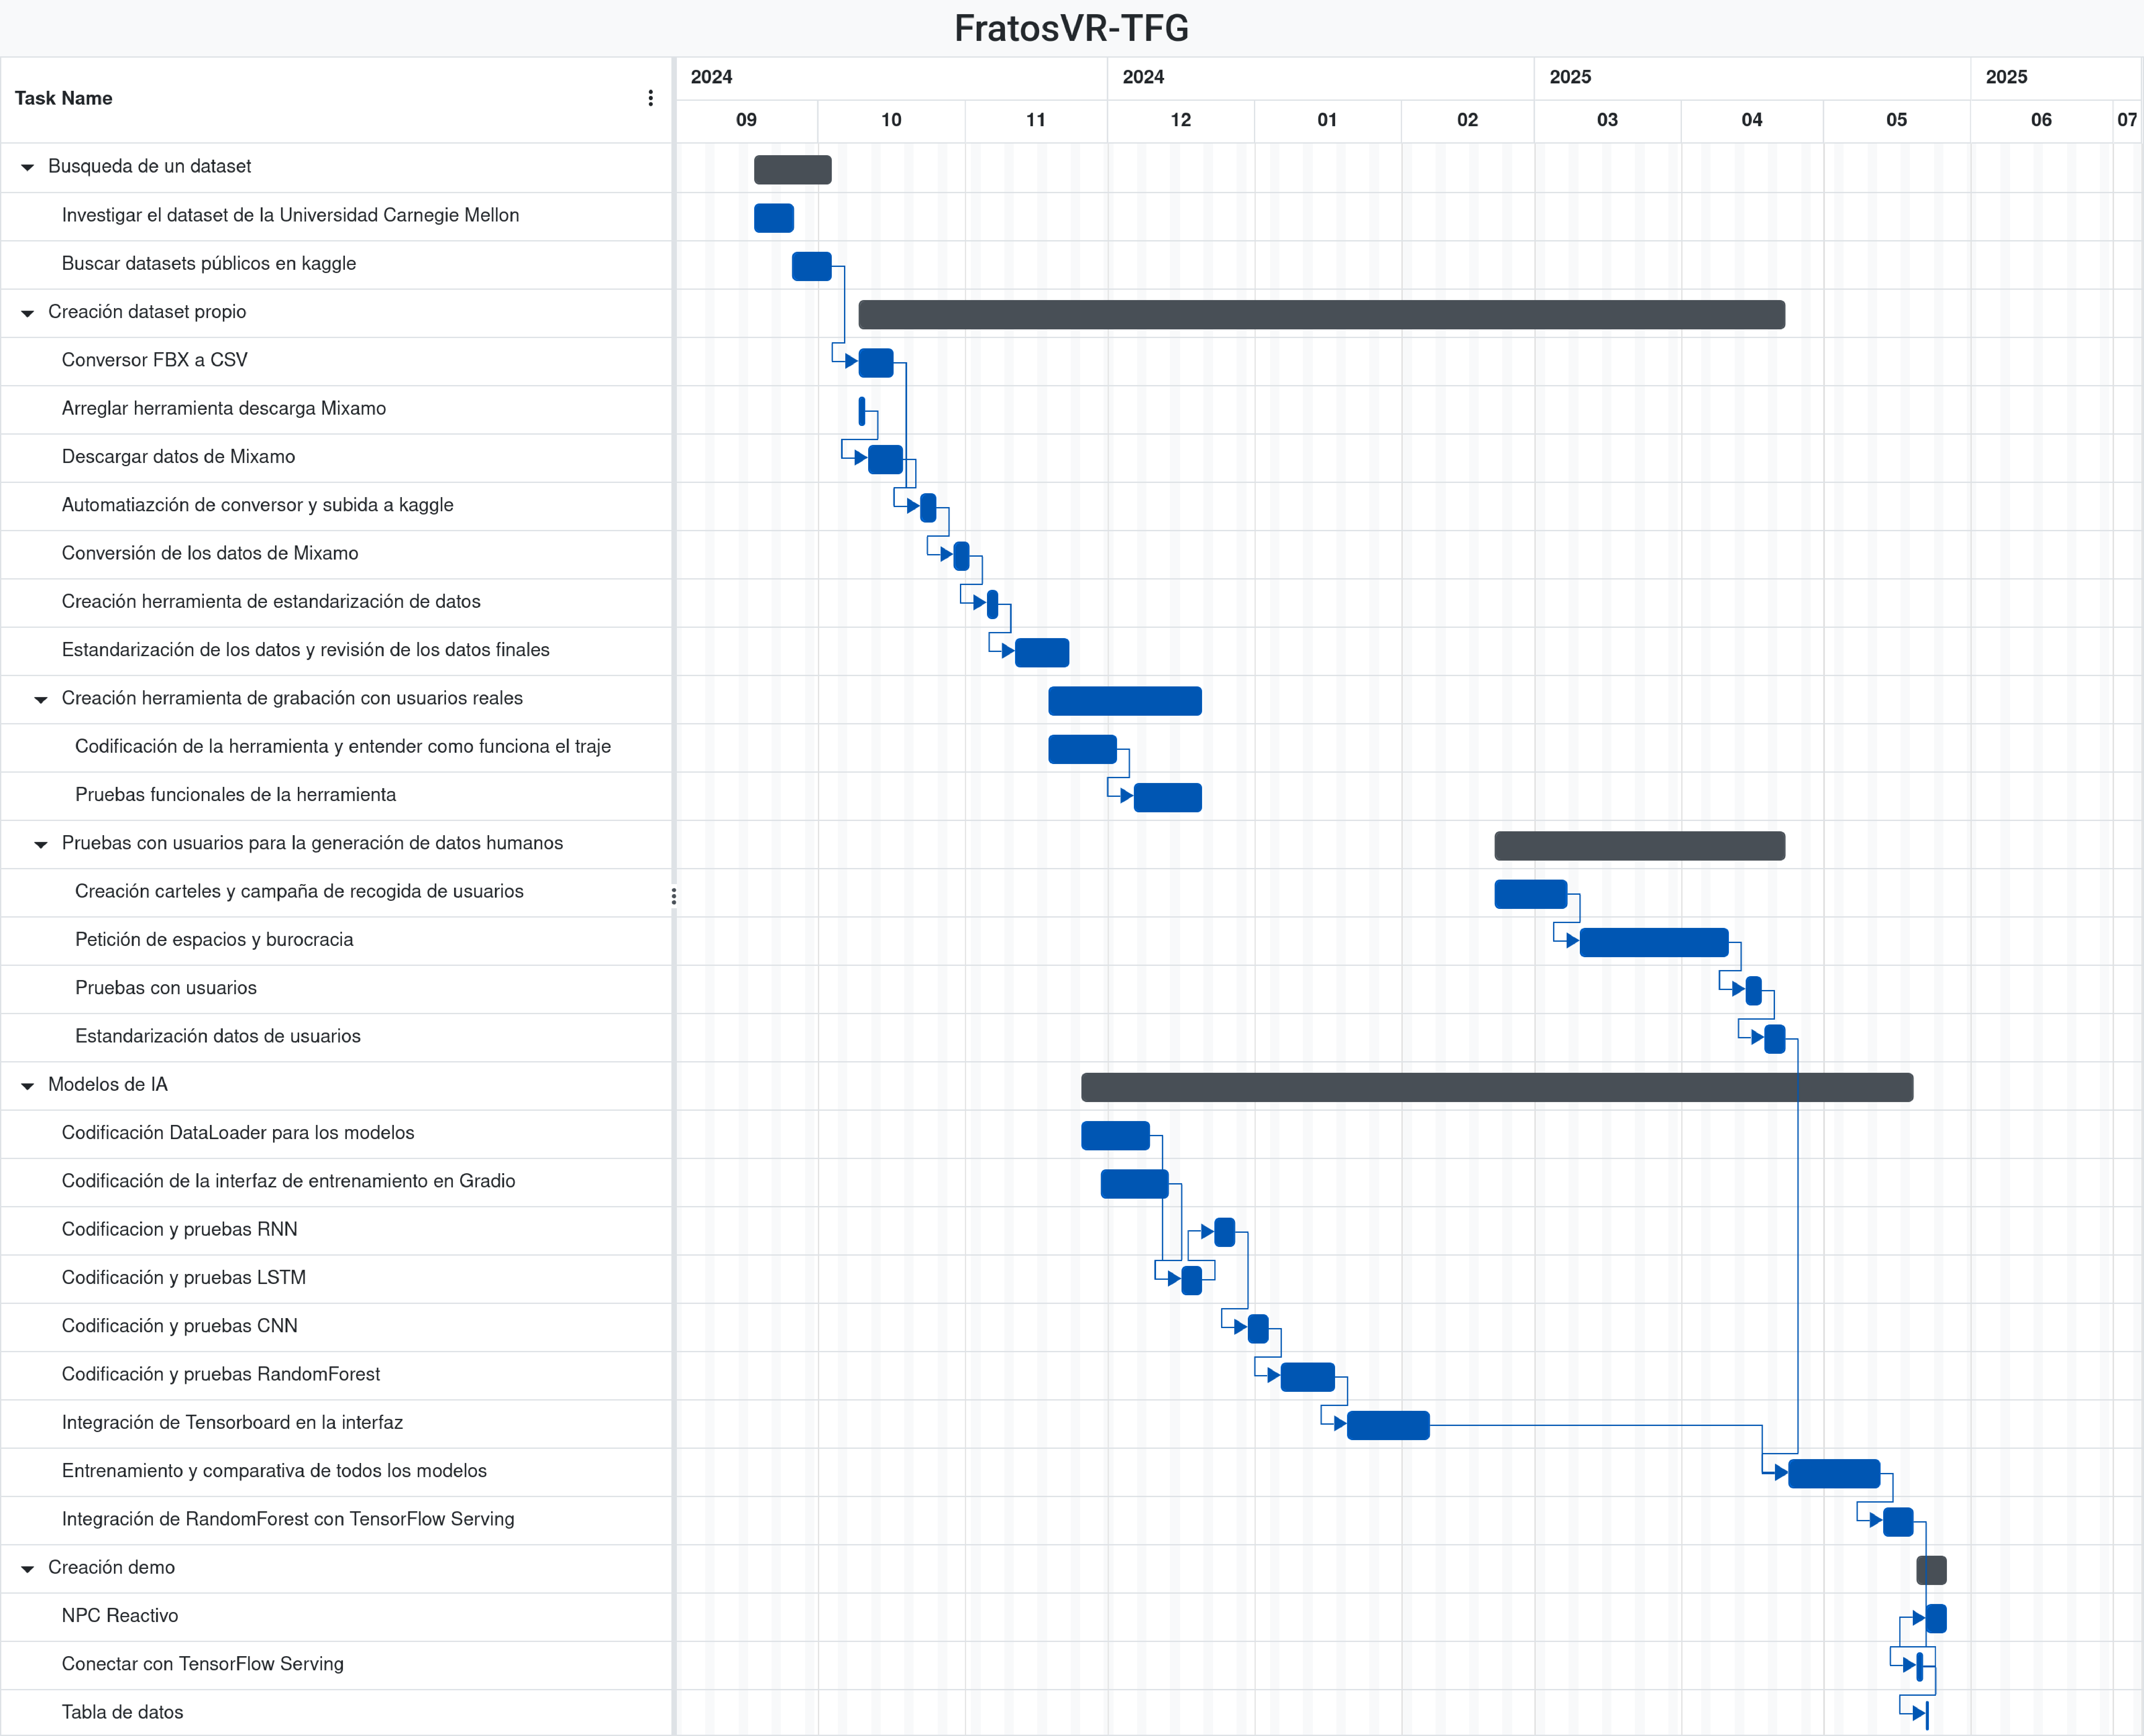
\includegraphics[width=0.91\textwidth]{Imagenes/Vectorial/Diagrama-gannt.pdf}
	\caption{Diagrama de Gantt del proyecto}
	\label{fig:diagrama-gantt}
\end{figure}

\section{Metodología}
Para el desarrollo de esta investigación, se utilizarán una serie de herramientas de libre acceso para todos los públicos y gratuitas, lo que facilita la reproducibilidad de los resultados obtenidos.
Desarrollo en SO Windows 11, lo más común en nuestro equipo y posibles usuarios?
Creación de la animación e integración del modelo en Unity versión 6000.3.2f1 (última versión disponible de soporte a largo plazo).
Lenguaje de programación:  \ttvar{C#} en unity para la recogida de datos y utilización del modelo, python para el entrenamiento.
Sentis como integración del modelo entrenado fuera en code.
Github para trabajo en equipo (basado en Git, control de versiones).
Github projects para la creación y asignación de tareas en iteraciones.
Google Drive como herramienta adicional de almacenaje para  apuntes de reuniones, pasos que damos.
Discord para llevar a cabo reuniones, a parte de las reuniones presenciales semanales.

\section{Estructura de la memoria (propuesta)}